\documentclass[tikz,border=10pt]{standalone}
\usepackage{circuitikz}
\usepackage{xcolor}
\usepackage{amsmath}
\usetikzlibrary{arrows}

\begin{document}
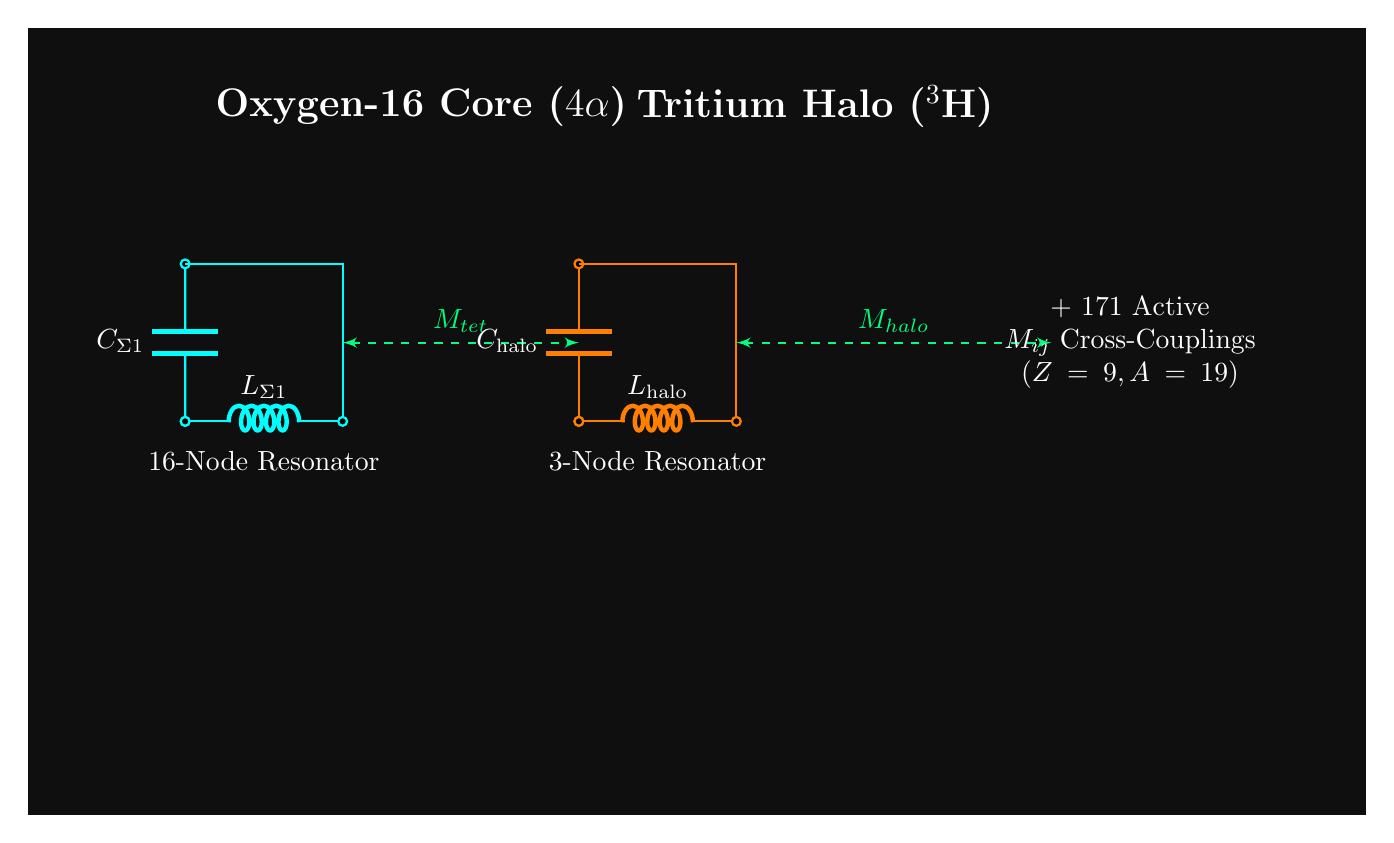
\begin{tikzpicture}[>=latex']

% Define neon-like glow colors
\definecolor{neonblue}{RGB}{0, 255, 255}
\definecolor{neongreen}{RGB}{0, 255, 128}
\definecolor{darkbg}{RGB}{15, 15, 15}
\definecolor{neonorange}{RGB}{255, 128, 0}

% Fill background
\fill[darkbg] (-5,-5) rectangle (12,5);

% OXYGEN-16 CORE (16 Nucleons)
\node[text=white, font=\bfseries\Large] at (0, 4) {Oxygen-16 Core ($4\alpha$)};

% Core Tank 1
\draw[neonblue, thick] (-3, 0) to[C, l=\color{white}$C_{\Sigma1}$, *-*] (-3, 2);
\draw[neonblue, thick] (-3, 0) to[L, l=\color{white}$L_{\Sigma1}$, *-*] (-1, 0) -- (-1, 2) to[short] (-3, 2);
\node[text=white] at (-2, -0.5) {16-Node Resonator};

% M_core coupling
\draw[<->, neongreen, thick, dashed] (-1, 1) -- (2, 1) node[midway, above] {$M_{tet}$};

% TRITIUM HALO (3 Nucleons)
\node[text=white, font=\bfseries\Large] at (5, 4) {Tritium Halo ($^3\text{H}$)};

% Halo Tank
\draw[neonorange, thick] (2, 0) to[C, l=\color{white}$C_{\text{halo}}$, *-*] (2, 2);
\draw[neonorange, thick] (2, 0) to[L, l=\color{white}$L_{\text{halo}}$, *-*] (4, 0) -- (4, 2) to[short] (2, 2);
\node[text=white] at (3, -0.5) {3-Node Resonator};

\draw[<->, neongreen, thick, dashed] (4, 1) -- (8, 1) node[midway, above] {$M_{halo}$};

% The 171 Matrix representation
\node[text=white, text width=4cm, align=center] at (9, 1) {+ 171 Active\\$M_{ij}$ Cross-Couplings\\($Z=9, A=19$)};

\end{tikzpicture}
\end{document}
